\documentclass[12pt,oneside]{book}
\usepackage{geometry}                		% See geometry.pdf to learn the layout options. There are lots.
\geometry{a4paper}                   			% ... or a4paper or a5paper or ... 
%\geometry{landscape}                		% Activate for for rotated page geometry
%\usepackage[parfill]{parskip}    		% Activate to begin paragraphs with an empty line rather than an indent
\usepackage{graphicx}				% Use pdf, png, jpg, or epsß with pdflatex; use eps in DVI mode
								% TeX will automatically convert eps --> pdf in pdflatex		
\usepackage{amssymb}

\usepackage[spanish]{babel}			% Permite que partes automáticas del documento aparezcan en castellano.
\usepackage[utf8]{inputenc}			% Permite escribir tildes y otros caracteres directamente en el .tex
\usepackage[T1]{fontenc}				% Asegura que el documento resultante use caracteres de una fuente apropiada.

\usepackage{hyperref}				% Permite poner urls y links dentro del documento

\title{Mi Juego Favorito}
\author{Javier Tibau}
%\date{}							% Activate to display a given date or no date

\begin{document}
\maketitle
\tableofcontents

\chapter{Introducción}
El libro a continuación es creado como una herramienta para el desarrollo de habilidades de edición colaborativa de documentos de texto plano. La herramienta que habilita dicha colaboración, en este taller, es Git pero podría ser reemplazada por otros sistemas de versionamiento.

\chapter{Los Juegos}

\include{juegos/Buscaminas}
\include{juegos/Dota2}
\include{juegos/Zelda}
\section{Gatos Gemelos}

\begin{figure}[htbp]
\begin{center}
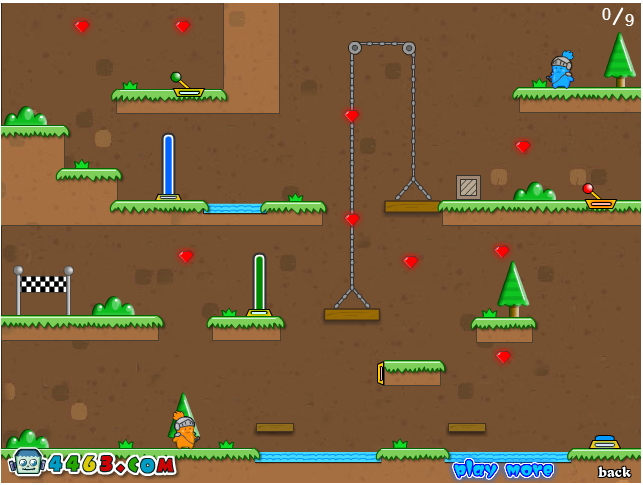
\includegraphics[width=.60\textwidth]{./imagenes/gatos1.png}
\caption{Gatos Gemelos}
\label{Gatos Gemelos}
\end{center}
\end{figure}
Gatos Gemelos \footnote{\url{http://ar.yayoye.com/twin-cat-online-game/22643/}} es un Juego en el que se deben mover a los personajes por la pantalla, como su nombre mismo lo dice son unos gatos gemelos, con los que iremos tratando de recoger diamantes y de lograr que interactúen entre ellos para superar los obstáculos.

\subsubsection{¿Por qué es uno de mis juegos favoritos?}
\begin{itemize}
\item[Tania Sánchez] En realidad no soy de esas personas que se vician con los juegos pero me llaman mucho la atención el tipo de juego que estimula el aprendizaje, me parece que este juego lo hace, ya que es un juego que se realiza en pareja en el que enseña el trabajo en equipo, a medida que avanzan los niveles va aumentando la dificultad del mismo, poniendo al usuario cada vez a pensar más en como vencer los obstaculos tomando en cuenta que un jugador debe ir a la par con el otro e irlo ayudando para juntos llegar a la meta, la dificultad del juego aparte de resolver como se debe avanzar, está en no olvidarse del compañero ya que aunque llegue uno de los dos solo a la meta no implicará que se pasará al siguiente nivel sino que deben llegar los dos juntos. 
\\
\\
Éste es un juego orientado más para niños pequeños para estimular el desarrollo intelectual y enseñarles el trabajo en equipo =).
\end{itemize}



\chapter{Conclusiones}
Cuales juegos fueron más populares y un breve razonamiento del porqué.

\end{document}  
